\documentclass[12pt, letterpaper]{article}

% %%%%%%%%% Packages %%%%%%%%%%
\usepackage[empty]{fullpage}
\usepackage{geometry}
\usepackage{fontawesome5}
\usepackage{ragged2e}
\usepackage{graphicx}
\usepackage{xcolor}
\usepackage{titlesec}
\usepackage[hidelinks]{hyperref}
\usepackage{tabularx}
\usepackage{enumitem}
\usepackage{multicol}
\usepackage[spanish]{babel}

% Settings
\geometry{lmargin=1cm,rmargin=1cm,tmargin=1cm,bmargin=1cm}
\urlstyle{same}

%% Section formatting
\titleformat{\section}{\centering\large}{}{0cm}{}[\titlerule]

%% News Commands
\newcommand{\CVName}[1]{\textbf{\Large #1} \\[3mm]}
\newcommand{\CVLocation}[1]{{\footnotesize \faMapMarked*} #1 \\}
\newcommand{\CVMobile}[1]{{\footnotesize \faMobile*} #1 \\}
\newcommand{\CVEmail}[1]{{\footnotesize \faEnvelope[regular] } \href{mailto:#1}{#1} \\}
\newcommand{\CVLinkedin}[1]{{\footnotesize \faLinkedin}\ \url{#1} \\}
\newcommand{\CVGithub}[1]{{\footnotesize \faGithub}\ \url{#1} \\}

\newcommand{\CVitem}[1]{
	\item \small{#1}  
}
\newcommand{\CVListStart}{\begin{itemize}[leftmargin=0cm, label={}]}
\newcommand{\CVListEnd}{\end{itemize}}
\newcommand{\CVSubHeading}[4]{
	\item \begin{tabular*}{19.5cm}[t]{l@{\extracolsep{\fill}}r}
		\textbf{#1} & #2 \\
		\small #3 & \small #4 \\
	\end{tabular*} \vspace{-8pt}
}
\newcommand{\CVItemizeStart}{\begin{itemize}[rightmargin=0.3cm, label={\tiny \textbullet}]}
\newcommand{\CVItemizeEnd}{\end{itemize}}


\begin{document}
% 	\begin{center}
% 	Fecha de elaboración: 1 de febrero de 2024 
% \end{center}
\begin{minipage}[c]{2.7cm}
	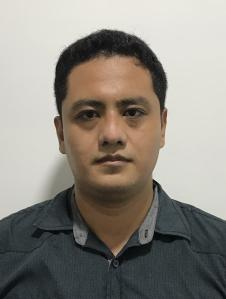
\includegraphics[width=2.5cm, height=3.5cm]{images/fotocv.jpg}
	\hfill
	\vrule
	\hfill
\end{minipage}
\begin{minipage}[c]{20cm}
	\vspace{4mm}
	\CVName{Edwin Enrique Pérez Rodríguez}
	\CVLocation{Tabasco, México}
	\CVMobile{9932885771}
	\CVEmail{edwin.epr.219@gmail.com}
	\CVLinkedin{https://www.linkedin.com/in/edwin-epr/}
	\CVGithub{https://github.com/EdHeny}
\end{minipage}

\section{Educación}
\CVListStart
\CVSubHeading{Maestria en Ciencia e Ingeniería de la Computación}{Agosto 2021 - Julio 2023}{Programa de Posgrados}{CDMX, México}
\CVItemizeStart
\CVitem{IIMAS UNAM}
\CVitem{Becario CONACHyT}
\CVitem{Tesis: Implementación de Métodos Numéricos para Resolver Sistemas de Ecuaciones  Lineales Mediante Estrategias de Cómputo de Alto Rendimiento.}
\CVitem{Avance de Tesis: 60 \%}
\CVitem{Fecha tentativa de obtención de grado: Junio 2024}
\CVItemizeEnd
\CVSubHeading{Licenciatura en Matemáticas}{Agosto 2016 - Junio 2020}{División Académica de Ciencias Básicas}{Tabasco, México}
\CVItemizeStart
\CVitem{UJAT}
\CVitem{Tesis: Resolución Numérica de la Ecuación de Poisson en 1D y 2D por el Método de Diferencias Finitas.}
\CVitem{Titulado}
\CVItemizeEnd
\CVListEnd
\section{Experiencia Profesional}
\CVListStart
\CVSubHeading{\small Ayudante de Profesor del Dr. Óscar Alejandro Esquivel Flores}{Agosto 2022 - Diciembre 2022}{IIMAS UNAM}{CDMX, México}
\CVItemizeStart
\CVitem{Técnicas de paralelización usando los lenguajes de programación Julia y C para alumnos de la Licenciatura en Ciencia de Datos. }

\CVItemizeEnd
\CVSubHeading{\small Ayudante de Profesor del M. en C. David Chaffrey Moreno Fernández}{ Enero 2023 - Junio 2023}{Facultad de Ciencias UNAM}{CDMX, México}
\CVItemizeStart
\CVitem{Elaboré e impartí un taller de Estructuras Avanzadas de Datos en Python para alumnos de la Facultad de Ciencias.}
\CVItemizeEnd
\CVListEnd
\section{Habilidades}
\CVListStart
\CVSubHeading{Idiomas}{}{}{}
\vspace{-15pt}
\CVItemizeStart
\begin{multicols}{3}
	\CVitem{Español (Nativo)}
	\CVitem{Inglés (Intermedio)}
\end{multicols}
\CVItemizeEnd
\CVSubHeading{Lenguajes de Programación}{}{}{}
\vspace{-15pt}
\CVItemizeStart
\begin{multicols}{4}
	\CVitem{C/C++}
	%\CVitem{Julia}
	\CVitem{Python}
	%\CVitem{MatLab}
	%\CVitem{Kotlin}
	\CVitem{Julia}
	%\CVitem{Bash}
\end{multicols}
\CVItemizeEnd
\newpage
\CVSubHeading{Bibliotecas de Cómputo de Alto Rendimiento}{}{}{}
\vspace{-15pt}
\CVItemizeStart
\begin{multicols}{3}
	\CVitem{MPI (conocimientos básico)}
	\CVitem{OpenMP (conocimientos básico)}
	\CVitem{CUDA (conocimientos básicos)}
\end{multicols}
\CVItemizeEnd
\CVSubHeading{Procesadores de Texto y Lenguajes de Marcado}{}{}{}
\vspace{-15pt}
\CVItemizeStart
\begin{multicols}{3}
	\CVitem{Microsoft Office Suite}
	\CVitem{Latex}
	\CVitem{Markdown}
\end{multicols}
\CVItemizeEnd
\CVSubHeading{Sistemas Operativos}{}{}{}
\vspace{-15pt}
\CVItemizeStart
\begin{multicols}{3}
	\CVitem{Linux}
	\CVitem{Windows}
\end{multicols}
\CVItemizeEnd
\CVListEnd
\section{Actividades Académicas}
\CVItemizeStart
\CVitem{Tomé el curso virtual <<Fundamentos de la modelación matemática: Un acercamiento a la  epidemiología matemática>> impartido por la Sociedad Mexicana de Computación Científica y  sus Aplicaciones, los días 25, 30 de junio y 2 de julio del 2020, con una duración de 5 horas.}
\CVitem{Presenté la ponencia <<Resolución Numérica de la Ecuación de Poisson en 2D>> en XII Foro de
	Matemáticas del Sureste llevado a cabo del 9 al 13 de septiembre de 2019 en Cunduacán,
	Tabasco.}
\CVitem{Tomé el curso «El método de elemento finito para la solución de la ecuación de calor» en el
	marco del XII Foro de Matemáticas del Sureste, con una duración de 4 horas.}
\CVitem{Presenté la ponencia «Resolución Numérica de la Ecuación de Poisson en 2D» en XXVIII
	Escuela Nacional de Optimización y Análisis Numérico llevado a cabo del 26 al 30 de agosto
	de 2019 en Zacatecas, Zacatecas.}
\CVitem{Participé en el equipo organizador del 51 Congreso Nacional de la Sociedad Mexicana de
	Matemáticas llevado a cabo del 21 al 26 de octubre de 2018 en Villahermosa, Tabasco.}
\CVitem{Participé con el cartel “Tratamiento óptimo del VIH al maximizar la respuesta inmune”, en el
	Congreso Sur-sureste de Matemáticas 2017 llevado a cabo del 20 al 24 de noviembre en
	Oaxaca, Oaxaca.}
\CVItemizeEnd
\end{document}
